\subsection{Concrete candidates and held-out SCIC-v2 evaluation}

\label{sec:v2-evaluation}

The revised study is archived separately from all earlier measurements. It uses PyTorch 2.13.0+cu126, Triton 3.7.1, Transformers 5.17.0, and vLLM 0.31.0 on A40 GPUs, with one CPU thread. No primary worker initializes a profiler.

The operator matrix contains 32 geometries: 23 training geometries and nine held-out square-width-2048/8192 geometries. Direct execution and static CUDA Graph replay, and one repeated weight versus six rotated weights, form separate domains. Each candidate has 50 warmups, 200 event samples, and five synchronized host batches of 40 calls; host-batch medians are the primary objective. Selection uses fresh three-warmup probes with five eight-call host batches.

Component validation uses three input seeds, unit and nonunit affine weights, and stress inputs. Both normalized output and residual require relative and absolute tolerances of $10^{-3}$ and relative L2 error at most $10^{-3}$. Numerical rejection and native fallback remain in the artifact. The pool minimum is an oracle over admitted implementations, not evidence that a rejected schedule is usable.

The HF operator series uses six independent processes on two A40 devices. After the other device failed the idle gate, the remaining random-model domains use five processes on physical GPU 1 and pretrained domains use three. These repetitions assess process variation on the available hardware; they are not five independent devices. Registration-failure control trials are archived and excluded; corrected controls are paired only where the same GPU/run and geometry have a completed optimized baseline.

Completed primary workers are: 6 HF-semantic operator workers, 5 vLLM-semantic operator workers, 5 unmodified legacy-dispatch workers, 5 random-model HF workers, and 3 pretrained HF workers. Stages without completed workers have no measured result.

\begin{table*}[t]
\centering\small
\caption{SCIC-v2 held-out comparison. Steady speed is full-calibration latency divided by revised-policy latency; preparation speed includes common compilation/validation and policy probes. Achieving a 30\% reduction requires preparation speed at least $1/0.7$. Domains are not pooled.}
\label{tab:v2-selection}
\begin{tabular}{llllrrr}
\toprule
Semantics & Execution & Weight reuse & Policy & Steady & Preparation & AI/no-AI \\
\midrule
HF & direct & same & v2 & 0.998 & 1.000 & 1.000 \\
HF & direct & same & no-AI & 0.998 & 1.000 & -- \\
HF & direct & rotated & v2 & 0.998 & 1.000 & 1.000 \\
HF & direct & rotated & no-AI & 0.998 & 1.000 & -- \\
HF & graph & same & v2 & 1.002 & 1.000 & 1.000 \\
HF & graph & same & no-AI & 1.002 & 1.000 & -- \\
HF & graph & rotated & v2 & 0.999 & 1.000 & 1.000 \\
HF & graph & rotated & no-AI & 0.999 & 1.000 & -- \\
vLLM & direct & same & v2 & 0.982 & 1.000 & 0.995 \\
vLLM & direct & same & no-AI & 0.987 & 1.000 & -- \\
vLLM & direct & rotated & v2 & 0.988 & 1.000 & 1.000 \\
vLLM & direct & rotated & no-AI & 0.988 & 1.000 & -- \\
vLLM & graph & same & v2 & 1.000 & 1.000 & 1.000 \\
vLLM & graph & same & no-AI & 1.000 & 1.000 & -- \\
vLLM & graph & rotated & v2 & 0.999 & 1.000 & 1.000 \\
vLLM & graph & rotated & no-AI & 0.999 & 1.000 & -- \\
\bottomrule
\end{tabular}
\end{table*}

The operator scan prepares every candidate to audit the pool. Its preparation column therefore accounts for a common exhaustive compilation/validation cost and measures search savings conditional on that protocol. It is not a measurement of cold, lazy deployment preparation. Full-model preparation records separately report the actual candidates compiled, validated, and probed, under the observed compiler-cache state.

In the HF-semantic training-only audit, split factors four and eight each retain 3 and 3 distinct numerically admitted geometries, respectively. Each candidate is fitted separately, so constant candidate-identity features do not supply additional shape information. Large leave-one-geometry-out residual margins often force expanded probing. This is a training-support and model-identifiability limitation, not evidence that arithmetic intensity determines the best schedule. The audit does not tune features or hyperparameters on held-out timings.

HF-semantic v2/full-calibration steady ratios (95\% process-bootstrap intervals), in direct/same, direct/rotated, graph/same, and graph/rotated order, are 0.9975 [0.9932, 1.0000], 0.9976 [0.9929, 1.0002], 1.0023 [0.9991, 1.0080], 0.9990 [0.9986, 0.9995].

vLLM-semantic v2/full-calibration steady ratios (95\% process-bootstrap intervals), in direct/same, direct/rotated, graph/same, and graph/rotated order, are 0.9818 [0.9759, 0.9876], 0.9880 [0.9872, 0.9887], 0.9998 [0.9994, 1.0004], 0.9994 [0.9978, 1.0006].

\begin{figure*}[t]
\centering
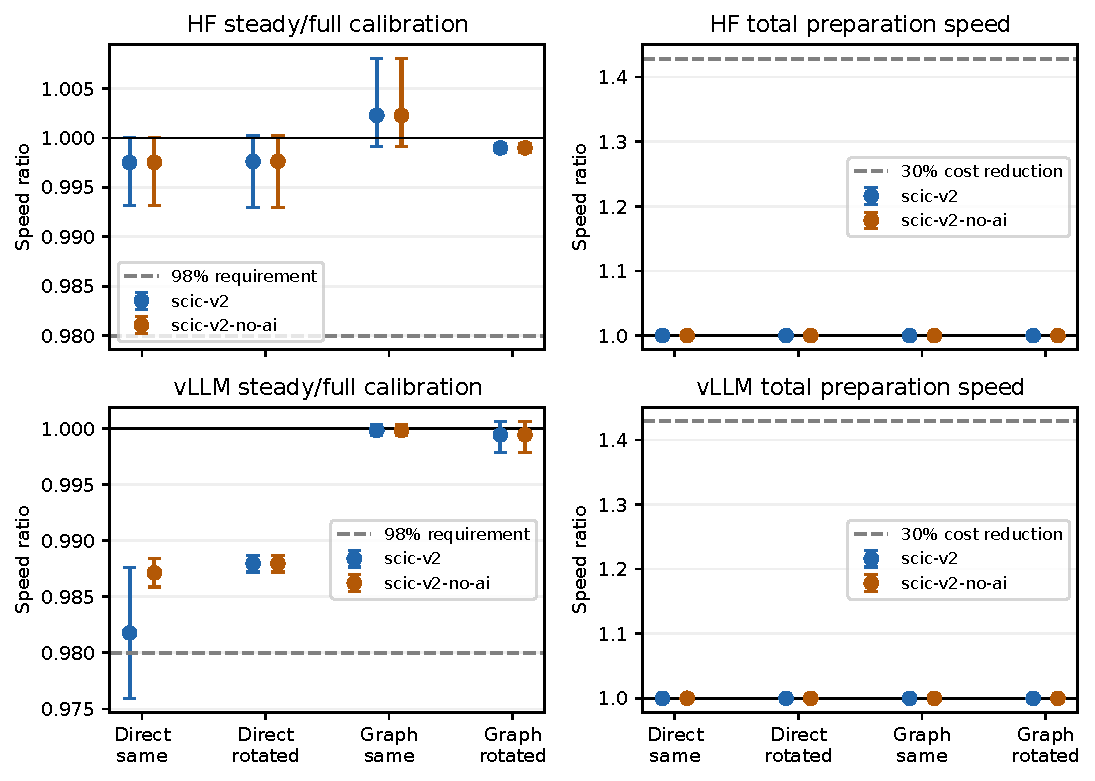
\includegraphics[width=\textwidth]{figures/fig_v2_selection.pdf}
\caption{Held-out steady performance and exhaustive-scan preparation accounting. Error bars are 95\% GPU/run bootstrap intervals. The horizontal thresholds apply separately to each execution/reuse domain.}
\label{fig:v2-selection}
\end{figure*}

Of 16 measured execution/reuse/semantic/policy domains, 0 meet both the 98\% steady-performance requirement and the 30\% total-preparation reduction requirement. Training-only analytical features are assessed against the otherwise identical no-AI policy. Probe reductions alone cannot establish that preparation is cheaper.

\paragraph{Full-model and serving validation}

The pretrained checkpoint is Qwen/Qwen3-0.6B at revision \texttt{c1899de289a04d12100db\allowbreak370d81485cdf75e47ca}, loaded in FP16 for every arm. Its attention output projection is rectangular, with $K=2048$ and $N=1024$, and is an external geometry validation rather than additional fitting data. Random-model HF workloads retain four batch/prompt combinations; pretrained HF uses batch-one/128 and batch-eight/2048. Every prefill and all 64 teacher-forced decode outputs are checked against the optimized original. The elementwise logits tolerance is $10^{-2}$; the additional strict relative-L2 gate is $10^{-3}$. A strict failure has no primary acceleration claim, even when elementwise checks pass and exploratory latency is recorded.

A separate diagnostic finds that compiling the random-weight original model itself can exceed the strict relative-L2 threshold against its eager form. This does not justify changing the threshold after observing candidate results. The artifact retains both the strict verdict and exploratory timing.

Actual vLLM generation uses 128 requests with 64 greedy output tokens each, six random-model workloads and four pretrained workloads. Full request token hashes, TTFT, ITL, and startup/preparation costs are recorded. To preserve vLLM's unbounded dynamic token dimension, serving freezes one candidate per layer from a declared 64-decode/one-prefill calibration mixture. This restriction prevents treating serving as validation of arbitrary per-shape dynamic routing. Matching token hashes establishes generation equivalence on these requests, not language-task accuracy.

\begin{table*}[t]
\centering\small
\caption{Full-system ratios against the optimized original. HF columns use strictly admitted logits; parenthesized counts give valid paired observations. Generation columns include only matching complete request hashes. Incomplete numerical or request coverage cannot support an aggregate acceleration claim.}
\label{tab:v2-systems}
\begin{tabular}{lrrrrrr}
\toprule
Policy & HF rand. prefill & HF rand. decode & HF trained prefill & HF trained decode & vLLM rand. & vLLM trained \\
\midrule
best-fixed & 1.005 (10) & 0.999 (10) & 1.004 (3) & 1.000 (3) & -- (0) & -- (0) \\
legacy & 0.780 (10) & 0.590 (10) & -- (0) & -- (0) & -- (0) & -- (0) \\
full calibration & -- (0) & -- (0) & -- (0) & -- (0) & -- (0) & -- (0) \\
scic-v2 & -- (0) & -- (0) & -- (0) & -- (0) & -- (0) & -- (0) \\
scic-v2-no-ai & -- (0) & -- (0) & -- (0) & -- (0) & -- (0) & -- (0) \\
\bottomrule
\end{tabular}
\end{table*}

Intervals use 5000 bootstrap resamples of independent GPU/run clusters, after averaging log ratios within each cluster; timer iterations are not independent replicates. A system acceleration claim additionally requires a ratio of at least $1.02\times$, a 95\% lower bound above one, and complete numerical/request coverage. Analytic cold traffic is not measured DRAM traffic, and pretrained inference is not a task-accuracy evaluation.

hf/best-fixed restores native functional endpoints in all layers/phases for 10 of 20 measured cases; 10 of these cases pass strict logits. Their timings do not establish a fused-candidate gain.

Random-model HF actual component-preparation speed relative to full calibration is 1.1676 [0.9660, 1.5901]; 0 paired cases also pass strict full-model logits in both arms. This descriptive preparation ratio does not establish valid system acceleration, and the observed compiler-cache state does not represent cold startup.

hf-pretrained/best-fixed restores native functional endpoints in all layers/phases for 3 of 6 measured cases; 3 of these cases pass strict logits. Their timings do not establish a fused-candidate gain.

Pretrained HF actual component-preparation speed relative to full calibration is 1.1979 [1.0117, 1.5833]; 0 paired cases also pass strict full-model logits in both arms. This descriptive preparation ratio does not establish valid system acceleration, and the observed compiler-cache state does not represent cold startup.
